\documentclass[a4paper]{article}

\usepackage[T1]{fontenc}
\usepackage{textcomp}
\usepackage{xcolor}
\usepackage{url}
\usepackage{stackengine}
\usepackage [english]{babel}
\usepackage [autostyle, english = american]{csquotes}
\usepackage{courier}
\usepackage{listings}
\usepackage{minted}
\usepackage{graphicx}
\usepackage{lmodern}
\usepackage{mathtools}
\usepackage{amsfonts}
\usepackage{float}



\lstset{
  basicstyle=\footnotesize\ttfamily,
  frame=single,
  numbers=left,
  captionpos=b
}


\begin{document}


\title{AI Assessed Exercise}

\author{Ross Meikleham 1107023m}

\maketitle


\section{Chapter 1 - Design}

\section{Chapter 2 - Theory}



\begin{figure}[H]
\begin{center}
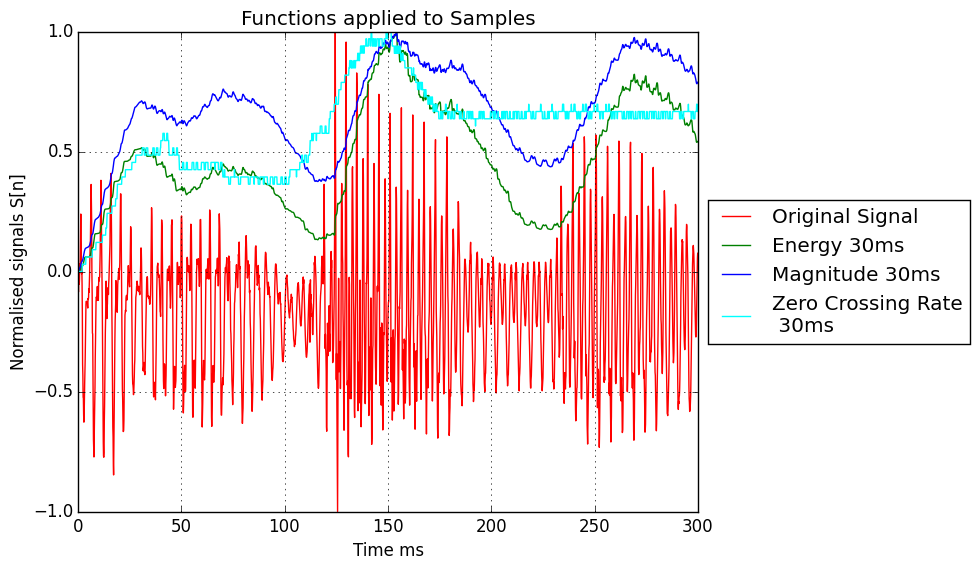
\includegraphics[width=\textwidth, height=\textheight, keepaspectratio]{../src/AI/Lab1/signals.png}
\caption{.}
\label{signals}
\end{center}
\end{figure}



\section{Chapter 3 - Experiments}


\begin{figure}[H]
\begin{center}
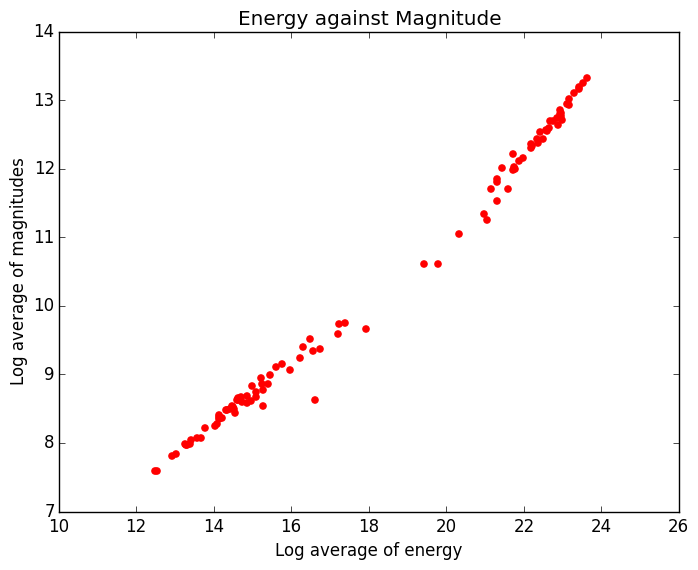
\includegraphics[width=\textwidth, height=\textheight, keepaspectratio]{../src/AI/Lab2/eam.png}
\caption{.}
\label{plot1}
\end{center}
\end{figure}


\begin{figure}[H]
\begin{center}
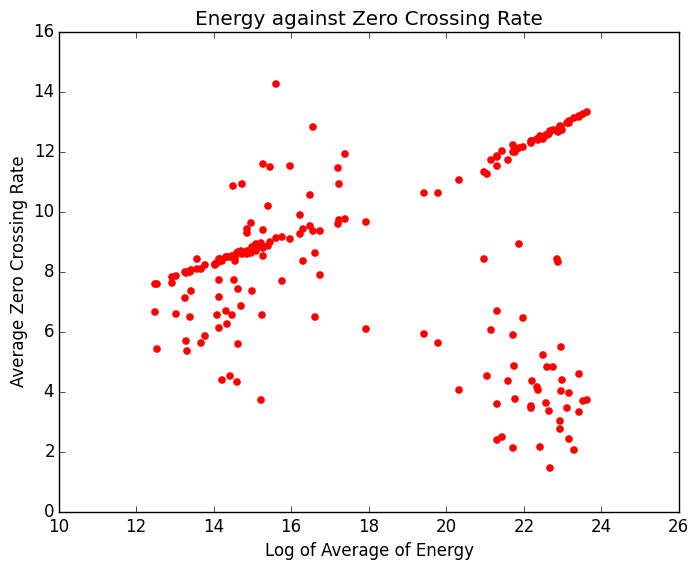
\includegraphics[width=\textwidth, height=\textheight, keepaspectratio]{../src/AI/Lab2/eac.png}
\caption{.}
\label{plot2}
\end{center}
\end{figure}


\begin{figure}[H]
\begin{center}
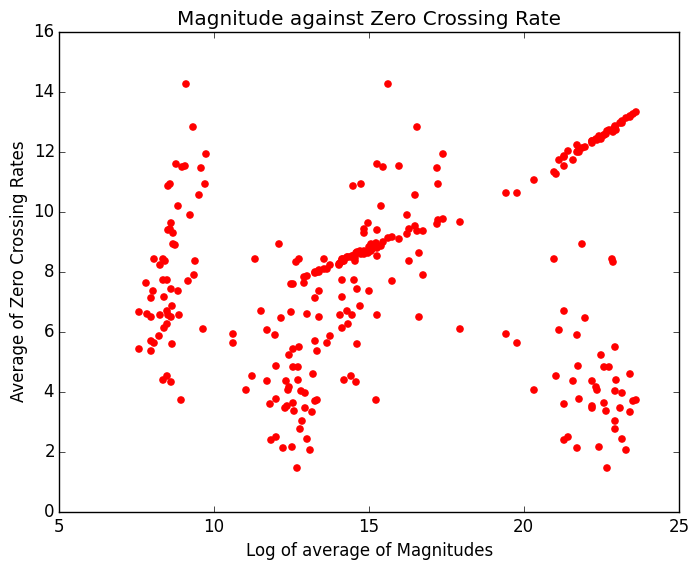
\includegraphics[width=\textwidth, height=\textheight, keepaspectratio]{../src/AI/Lab2/maz.png}
\caption{.}
\label{plot3}
\end{center}
\end{figure}

\newpage

\appendix

\section{Lab1 Processing Code} (Haskell)

\subsection{Lab1.hs}
\inputminted{haskell}{../src/AI/Lab1/Lab1.hs}

\subsection{Main.hs}
\inputminted{haskell}{../src/AI/Lab1/Main.hs}

\section{Lab1 Plotting Code} (Python)
\inputminted{python}{../src/AI/Lab1/plotting.py}


\section{Lab2 Processing Code (Haskell)}

\subsection{Lab2.hs}
\inputminted{haskell}{../src/AI/Lab2/Lab2.hs}

\subsection{Main.hs}
\inputminted{haskell}{../src/AI/Lab2/Main.hs}


\section{Lab2 Plotting Code (Python)}
\inputminted{python}{../src/AI/Lab2/plotting.py}



\end{document}
